\documentclass[times, 10pt,twocolumn]{article} 
\usepackage{latex8}
\usepackage{times}

%\documentstyle[times,art10,twocolumn,latex8]{article}

%------------------------------------------------------------------------- 
% take the % away on next line to produce the final camera-ready version 
\pagestyle{empty}

\usepackage[utf8]{inputenc}
\usepackage{graphicx}
\usepackage{url}
\usepackage{float}
\usepackage{times}    
\usepackage{multirow}    
\usepackage{listings}   
\usepackage{times}     
\usepackage{paralist}    

\usepackage{listings}
\usepackage{keyval}  
\usepackage{color}
\definecolor{listinggray}{gray}{0.95}
\definecolor{darkgray}{gray}{0.7}
\definecolor{commentgreen}{rgb}{0, 0.4, 0}
\definecolor{darkblue}{rgb}{0, 0, 0.4}
\definecolor{middleblue}{rgb}{0, 0, 0.7}
\definecolor{darkred}{rgb}{0.4, 0, 0}
\definecolor{brown}{rgb}{0.5, 0.5, 0}


\lstdefinestyle{myListing}{
  frame=single,   
  backgroundcolor=\color{listinggray},  
  %float=t,
  language=C,       
  basicstyle=\ttfamily \footnotesize,
  breakautoindent=true,
  breaklines=true
  tabsize=2,
  captionpos=b,  
  %numbers=left, 
  %numberstyle=\tiny
}

\title{Reliable Replica-Exchange Simulations of Biomolecular Systems
  on Production Distributed Environments using SAGA-CPR and Migol}
%  Computational Grids using SAGA-CPR and Migol}

\author{
  Andr\'e Luckow$^{1}$, Shantenu Jha$^{2,3}$, Joohyun Kim$^{2}$, Andre Merzky$^{2}$ and Bettina Schnor$^{1}$\\
  \small{\emph{$^{1}$Institute of Computer Science, Potsdam University, Germany}}\\
  \small{\emph{$^{2}$Center for Computation \& Technology, Louisiana State University, USA}}\\
  \small{\emph{$^{3}$Department of Computer Science, Louisiana State University, USA}}\\
}

%\date{}

\def\acknowledgementname{Acknowledgements}
\newenvironment{acknowledgement}%
{\section*{\acknowledgementname}%
\parindent=0pt%
}

\bibliographystyle{plain}

\newcommand{\kimnote}[1]{ {\textcolor{green} { ***JK: #1 }}}
\newcommand{\alnote}[1]{ {\textcolor{blue} { ***AL: #1 }}}
\newcommand{\amnote}[1]{ {\textcolor{magenta} { ***AM: #1 }}}
\newcommand{\jhanote}[1]{ {\textcolor{red} { ***SJ: #1 }}}

\begin{document} 


\maketitle    

\begin{abstract}
  There exist a class of scientific applications for which utilizing
  distributed resources is critical for a reduced time-to-solution for
  the problem at hand. However, a major challenge in a dynamic
  distributed enviroments with thousands of machines connected to each
  other is fault tolerance. The more resources and components, i.e.,
  degrees-of-freedom, that are involved, the more complicated and
  error-prone the system becomes.  We discuss one specific example of
  an application -- Replica Exchange simulations of biomolecular
  systems -- where utilizing as many (often heterogenous) distributed
  resources as possible, is critical for the effective solution of the
  scientific problem.  Thus a mechanism to co-exist and handle the
  fault-tolerance inherent in dynamic distributed systems is
  required. In this paper, we discusss the design, development and
  deployment of an unique framework to support fault-tolerant
  distributed simulations; critically our framework is scalable,
  general purpose and extensible. Our framework has two primary
  components: SAGA and Migol.  SAGA is a high-level programmatic
  abstration layer that provides an interface for the major
  distributed functionality required for application development; we
  provide details of a newly developed functionality in SAGA -- that
  of Checkpoint and Recovery. Migol is an adaptive Grid middleware,
  which addresses the fault tolerance of Grid applications and
  services by providing the capability to recover applications from
  checkpoint files transparently.  In addition to describing the
  design of the SAGA CPR package, the integration of the CPR adaptor
  with the Migol infrastructure, we outline our experiences with
  running a large scale, general-purpose, SAGA-CPR based
  Replica-Exchange application in a production distributed
  environment.

  % In addition to providing details of our implementation, we discuss
  % why our approach is unique.  SAGA~\cite{SAGA_Goodale06a} provides
  % a standardized, application-level API for common Grid scenarios,
  % e.\,g.\ the management of files and jobs. The new SAGA Checkpoint
  % Recovery (CPR) package addresses checkpointing and the automatic
  % recovery of Grid applications. In this paper, we describe the
  % design of the SAGA CPR package, the integration of the CPR adaptor
  % with the Migol infrastructure, and our experiences with running a
  % large scale SAGA CPR based task farming application in a real Grid
  % environment.
    
  % The aim of this paper is, i) to couple the SAGA and Migol
  % frameworks, ii) to provide a proof of concept implementation of
  % the replica exchange method that uses the SAGA/Migol frameworks,
  % iii) to show the validity, scalability and extensibility of this
  % approach by attempting the simulation of a large model system.
\end{abstract}



\Section{Introduction}
                           
Grid computing envisions the sharing of compute, network, data and
software resources across multiinstitutional virtual organizations
(VOs). Writing applications that are able to orchestrate heterogeneous
resources across virtual organizations (VO) is a complex task.  Several 
classes of applications, which are well suited for loosely
coupled Grids, exist; arguably the best known and most commonly used ones are
task farming applications. Despite the simple nature, many problems
can be solved with such a model, e.\,g.\ parameter studies found in
many sciences or Monte Carlo simulations. More
complicated, but possibly more interesting than {\it pleasingly
  distributed} applications, is the class of applications that are
essentially loosely-coupled, but with a small level of coupling
between the tasks.   A class of algorithms that belongs to this category are
\emph{Replica Exchange Molecular Dynamics (REMD)}~\cite{hansmann,Sugita:1999rm} simulations.
% Replica Exchange~\ref{repex1, repex2} simulations  %reference does not exist in bib
% are a class of algorithms that belong to this category.
% Algorithms that can effectively utilize distributed computing
% infrastructures are often different to those that utilize canonical
% high end computers.  
% Replica exchange (RE) methods~\cite{SPdynamics,
%   pande_bj03} are a class of algorithms that can utilize distributed
% computing infrastructure  
Such simulations are used to understand important physical
phenomena -- ranging from protein folding dynamics to conformational
configuration changes.

The \emph{Simple API for Grid Applications (SAGA)}~\cite{saga_gfd90}
provides a straightforward API for developing loosely coupled data and/or task
parallel applications.
% The framework provides an standardized, easy-to-use 
% API for applications to efficiently utilize Grid infrastructures. 
SAGA offers a standardized, easy to use API for utilizing Grid
infrastructures. The API supports e.\,g.\ the management of Grid jobs,
file transfers and replicas. Thus, SAGA is ideally suited to provide
the orchestration of the of replica exchange simulations across
distributed infrastructure.
                                                         
In replica exchange simulations, there is a need to occasionally attempt an exchange
between pairs of replicas; the pairing of replicas is also not a
constant and is dynamically determined. However, once the pair of
replicas has been established, a delay or loss of one replica will
stall the other replica. In the worst case, a single failing task can
render the entire computation worthless.
\emph{Migol}~\cite{schnorLuckow08} provides a fault tolerant Grid
middleware, which supports the discovery and allocation of resources
as well as the transparent starting, monitoring and recovery of tasks in the Grid.          



This paper describes In the full paper, we will extensively  describe the design of the SAGA CPR API and the implementation 
of the Migol adaptor. Further, we will present our experiences with deploying  
the REMD application in a Grid environment.
This paper describes how using the Checkpoint\,\&\,Recovery package
(CPR) of the SAGA API, Migol's fault tolerance can be provided to the
class of Replica Exchange applications.   

\jhanote{We need to compare our approach with i) WISDOM and ii)
  Folding@HOME}             

\alnote{Several project, such as Folding@home~\cite{folding} and Wisdom~\cite{wisdom}, rely on distributed infrastructures for computational biology and chemistry. While Folding@home utilizes a similar replica exchange algorithm~\cite{PhysRevLett.86.4983} 
to effectively parallelize simulations, it is based on BOINC~\cite{1033223}, a cycle scavenging infrastructure. 
In contrast, multipurpose Grids as the TeraGrid, which provide a dedicated runtime environment for applications with different characteristic, e.\,g.\ loosely coupled, tightly coupled and data-intensive applications, desktop Grids rely on volunteers. This kind of environment is only suitable for loosely coupled applications. Multipurpose Grids have several advantages: Issues as trust and security are well researched. Further, it is possible to run larger application chunks. The REMD manager splits an scenario into multiple parts -- each part can be represented by a MPI application utilizing up to 32 nodes. \\  
The Wisdom project utilizes the EGEE infrastructure for molecular docking simulations used e.\,g.\ for evaluation of drugs. While this application has a similar high throughput characteristic, the project is currently tied to the gLite~\cite{glite2008} Grid middleware.                      \\                             
In contrast to Wisdom and Folding@home, our approach is not restricted to a specific Grid middleware -- by utilizing the SAGA standard the REMD manager can easily utilize resources managed by different Grid platforms. SAGA provides a well-defined abstraction, which is capable of handling both scenarios. Using this approach the application can easily used with different middleware platforms, e.\,g.\ Folding@home could then be deployed on a BOINC infrastructure as well as on a multipurpose Grid, such as TeraGrid.                                                                                                                                                         
}

\alnote{Should we add some  details regarding  the scientific results of WISDOM and Folding@home and how they differ from
our REMD with NAMD? Or are we just comparing the Grid infrastructure?
}  
                       



\jhanote{The important message, which we need to repeat and repeat yet
  again: our approach is i) scalable over different distributed
  environments of different size (not like folding@home); ii) general
  -- usable over TG, DEISA, etc. unlike the WISDOM approach which is
  tied to EGEE; iii) extensible -- we can do Replica Exchange but we
  can also do other applications with this approach. We need to point
  that the ability to do all of the above arises from the use of the
  correct programmatic abstractions; let the systems/middleware do
  what middleware/systems do best (Migol); let users do what users do
  best!}

\jhanote{We need to address: ``Why SAGA and Migol?'' here in the
  opening section}


\Section{REMD Simulation with NAMD}   

REMD/NAMD background

Task management framework  / Python Experience etc.

...                                  


\Section{Migol: A Fault Tolerant Service Framework}     
\label{sec:migol}

\begin{figure*}[t]
            \centering
                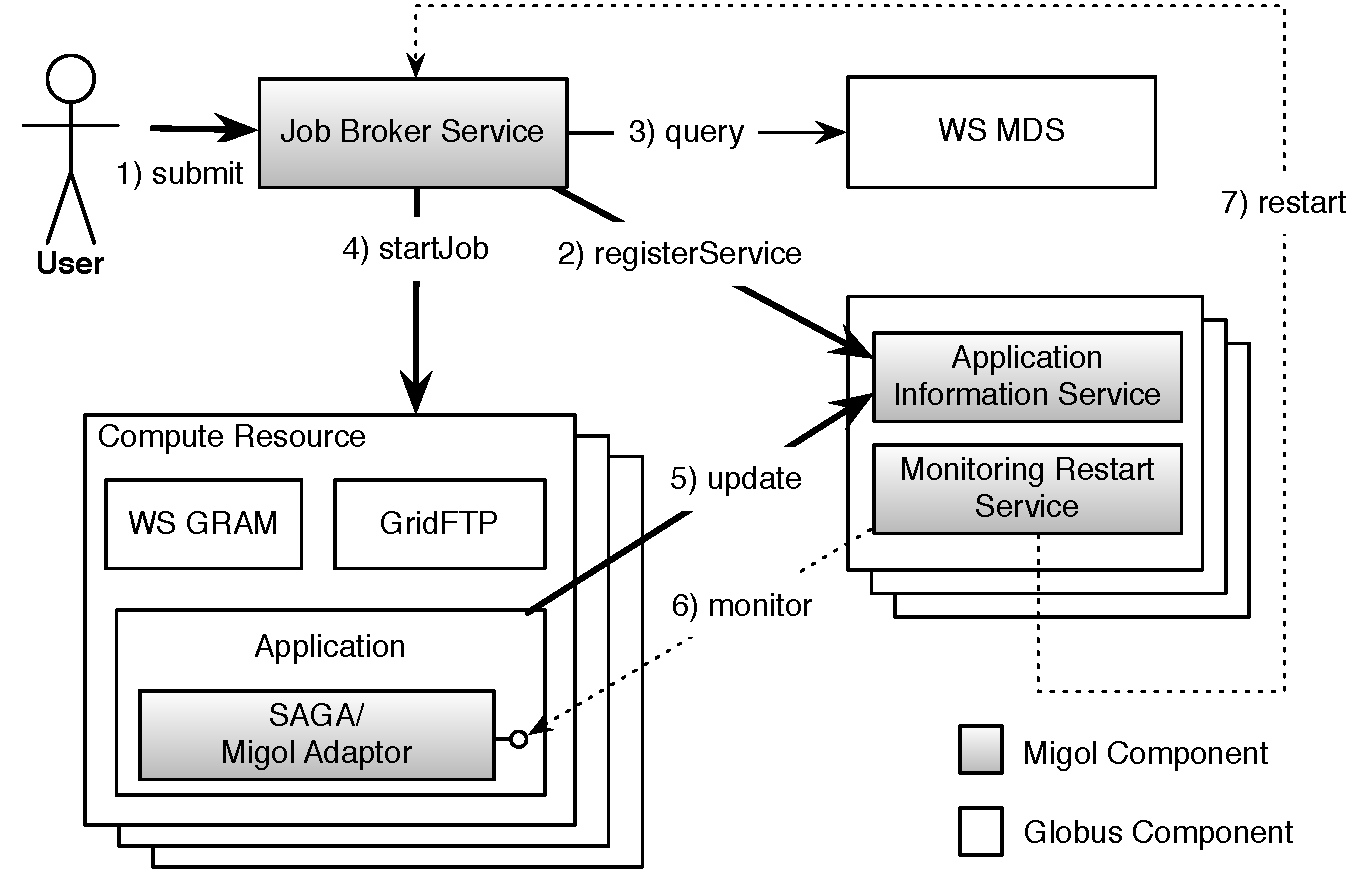
\includegraphics[width=0.7\textwidth]{migol_architecture}
            \caption{Migol Service Architecture and Interactions}
            \label{fig:migol_architecture}
\end{figure*}           


Migol guarantees the correct and reliable exe\-cution of applications or tasks even in
the presence of  failures. The framework is based on the Globus Toolkit 4. 
Figure~\ref{fig:migol_architecture} shows the current Migol architecture and 
the interactions between the different services.

The fundamental metadata model of Migol is the \emph{Grid Service Object (GSO)} schema,
which defines a generic and extensible information model for
describing Grid applications.  
%When an application is
%started, a Grid Service Object (GSO), which describedis created. 
A GSO stores all relevant information about an application: resource requirements,
the location of binaries and checkpoint files, global unique identifier (GUID),
etc.

Grid Service Objects for all running applications are stored in 
the {\em Application Information Service (AIS)}. 
Applications can register and update service metadata, 
such as files, machines etc.\ through Grid Services Objects. 
To avoid a single point of failure, the AIS is replicated using a ring-based
replication protocol, which ensures  the consistency of the stored data
(see~\cite{Luckow:2008ys} for more details).
%TODO plugin arch erläutern

Figure~\ref{fig:migol_architecture} shows the current Migol architecture and
the interactions between the different services.  Applications are
started using the {\em Job Broker Service (JBS)} (message 1 in 
Figure~\ref{fig:migol_architecture}). Before a job
submission, the JBS must register the GSO of the application at the AIS (message 2).
Resource discovery is performed through the WS MDS~\cite{schopf06},
which aggregates data of different services, e.\,g.\ the Network
Weather Service (NWS)~\cite{NWS99} (message 3).  Available resources are matched
by the JBS according to the requirements of the application. To better plan the execution of 
an application the JBS relies on advance reservation. The JBS tries to reserve a slot on all suitable
resources. All reservations are ranked based on a shortest expected
delay strategy~\cite{Jeske:2007wj}.  For conducting advance reservations and for job executions the
\emph{Advance Reservation Service (ARS)} is used (message 4).
             
To ensure the availability of the application state even in case of a failure, 
checkpoints can be replicated to another site  using the \emph{Checkpoint Replication Service
(CRS)} (message 6).  The CRS offers features such as the automatic discovery and selection of storage resources, 
the management of the data transfer and the detection of new file versions. 
The CRS uses an adaptive strategy to determine replication  targets respectively to select a replica for a
job restart.


Fault tolerance requires at least two basic mechanisms: failure
detection and recovery. To detect failures, the \emph{Monitoring and Restart Service (MRS)}
periodically checks all services registered at the AIS using an
application-level monitoring mechanism (message 8). In case the MRS discovers an inactive
application due to a timeout, it initiates a restart respectively a migration using the
Job Broker Service (message 9).  
          
For recovery, Migol relies on 
application-level checkpointing, i.\,e.\ applications have to be
written to accommodate checkpointing and restart. 
Each time a checkpoint is witten, the application has to update
its Grid Service Object at the AIS (message 5). 

To support an automatic recovery, Grid applications must be able to interact with the Migol infrastructure:
\begin{itemize}
    \item The application must register checkpoint and job metadata with the infrastructure.
    \item The infrastructure must be able to externally monitor the application.
    \item The infrastructure must be able to externally notify the application and trigger the saving of a checkpoint.
\end{itemize}  
The Simple API for Grid Applications (SAGA) provides a feature rich programing abstractions. The described functions 
can be  provided via the new SAGA Checkpoint Recovery API. In addition, SAGA provides  
various other APIs for supporting file transfer, RPC communication etc., which Grid applications can benefit of.                           


\Section{SAGA Checkpoint Recovery API}
                                                                                                         
The SAGA CPR package provides a clean abstraction for starting,
monitoring and recovering of checkpoint-restartable jobs.
% The package was inspired by the GridCPR~\cite{gridcpr} architecture and Migol.           
Using SAGA CPR, applications can register checkpoint and job metadata with the infrastructure. 
Further, the API provides support for starting applications, triggering of checkpoints and recoveries.  

For execution and management of CPR jobs, SAGA defines a CPR job. The management of 
CPR jobs is similar to regular jobs: A job is defined by a job description. In contrast to normal jobs, 
CPR jobs require  two job descriptions -- one for starting and another one for restarting the application.
Jobs are started using the job service. In addition to the normal job controls, a CPR job can be queried for checkpoint metadata, and 
it can be explicitly checkpointed or recovered. Listing~\ref{lst:saga_job_start} shows the starting of a CPR enabled job.

\begin{lstlisting}[style=myListing, caption={SAGA CPR: Starting a Job with CPR Support},  label={lst:saga_job_start}]
saga::cpr::service js; 
saga::cpr::description jd_start;
saga::cpr::description jd_restart;
//file out job description
...
//submit job  
saga::cpr::job job = js.create_job (jd_start, jd_restart);
job.run();
\end{lstlisting}
    
A major building block for fault tolerant system is failure detection. In general, fault detection is done by a monitor process, 
which periodically sends keep-alive messages to applications. To monitor applications, the application must provide a communication endpoint.
Listing~\ref{lst:saga_init_service} shows how a CPR application can connect to the CPR infrastructure. During instantiation of the \texttt{saga::cpr::service} object the adaptor is able to setup a monitoring thread (see section~\ref{sec:saga_cpr_migol_adaptor}). Using the \texttt{saga::cpr::self} object an application can obtain metadata about the current job from the application.                                                                               
\begin{lstlisting}[style=myListing, caption={SAGA CPR: Initialize Migol Session}, label={lst:saga_init_service}]
saga::cpr::service service (saga::url ("migol://gridhub.cct.lsu.edu:8443/wsrf/services/migol/AIS-JGroups"));
saga::cpr::self = service.get_self ();
\end{lstlisting}
      
After start of a CPR job, the job can be monitoring using the \texttt{job.get\_state()} method. Figure~\ref{fig:cpr-statemodel} shows the CPR state model. In the current implementation the \emph{recovering} state is introduced as detail substate of the state \emph{failed}.
\begin{figure}[th]
    \centering
        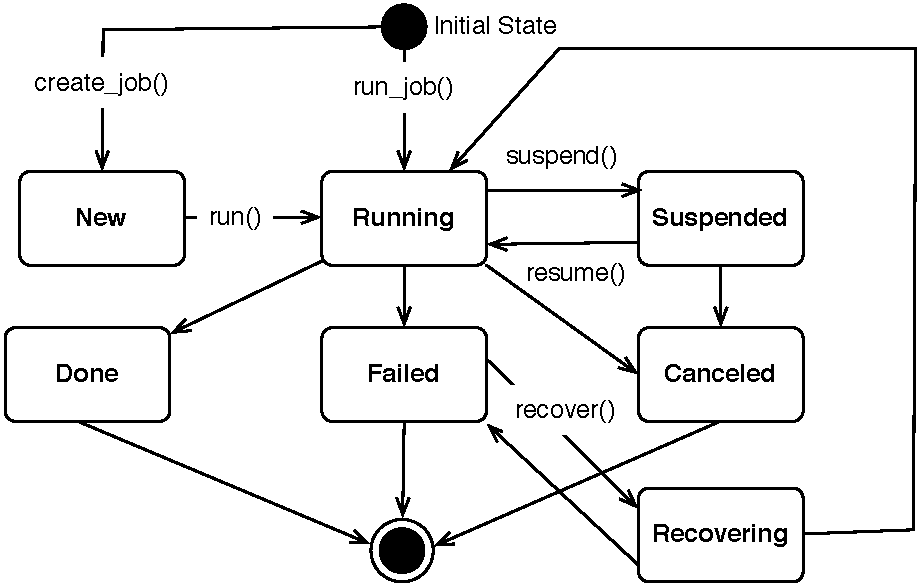
\includegraphics[width=0.48\textwidth]{cpr-statemodel.pdf}
    \caption{SAGA CPR State Model}
    \label{fig:cpr-statemodel}
\end{figure}
                               

For the management of checkpoint metadata the SAGA CPR API use the namespace paradigm to hierarchically 
organize files and directories. Checkpoint directories are 
used to group checkpoints. Parallel applications often write one checkpoint per 
processor, i.\,e.\ in case of $n$ processors a CPR checkpoint
would consists of $n$ files. Thus, a CPR checkpoint is designed as container 
for multiple physical or logical files. Listing~\ref{lst:saga_chkpt_reg} demonstrates how an application task registers a single checkpoint file with the CPR implementations.     
\begin{lstlisting}[style=myListing, caption={SAGA CPR: Register Checkpoint with Migol}, label={lst:saga_chkpt_reg}]
saga::cpr::checkpoint remd_chkpt("remd_chkpt");
remd_checkpoint.add_file(saga::url("gsiftp://queenbee.loni.org/work/remd/remd_chkpt.dat"));
\end{lstlisting}

In the following different implementation issues regarding the Migol SAGA adaptor are discussed.

\Section{SAGA CPR Migol Adaptor}  
\label{sec:saga_cpr_migol_adaptor}
                  
Naming: GUID - saga job id mapping

gsoap embedded web server as monitoring endpoint


\Section{Experiences with REMD}
\label{sec:exp}       

        
%do we use checkpoints or do we automatically restart the task
Figure~\ref{fig:saga-taskfarming} gives an overview about the task farming scenario. All tasks are
distributed using a script and Migol's Job Broker Service.
%  Each worker will compute a certain 
% variation of the graph network. Depending on the graph size, the runtime of a single task  can 
% be as high as \textbf{TODO}  days. 
To enable the monitoring of a tasks, each task must initialize a \texttt{saga::cpr::service} object 
before starting the computation.  Then, the Migol adaptor starts and registers the monitoring endpoint. 
%TODO what is the task size/runtime of a single task
The MRS can now monitor the application.  For error detection we use a timeout of \textbf{xx} minutes.
\begin{figure*}[t]
    \centering
        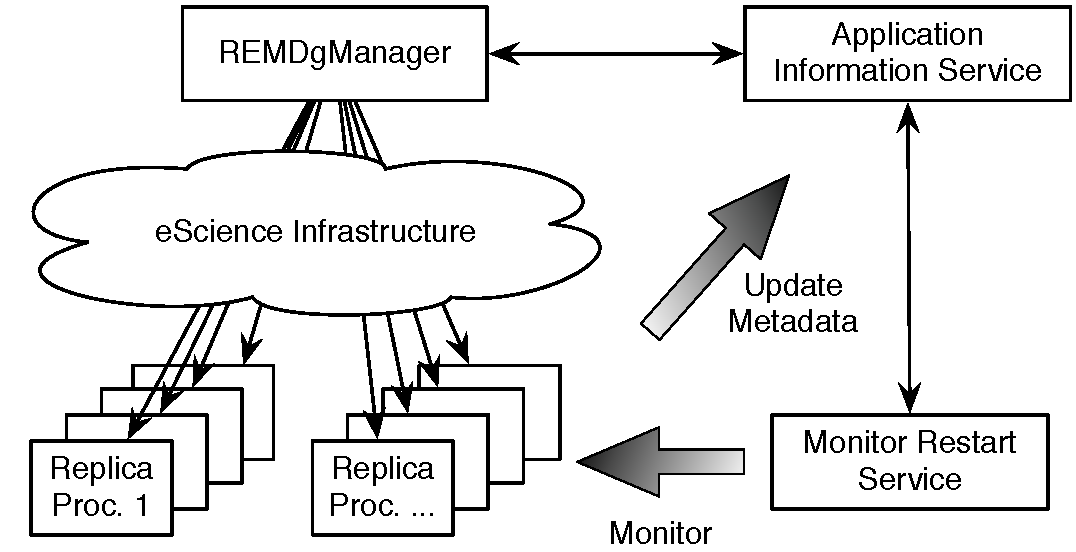
\includegraphics[width=0.6\textwidth]{saga-taskfarming}
    \caption{Fault Tolerant Task Farming Scenario}
    \label{fig:saga-taskfarming}
\end{figure*} 

The REMDgManager was functionally tested on the LONI Grid. The following aspects are from interest:
\begin{itemize}
    \item \textbf{Speedup}: This test determines how much faster the Grid-enabled replica exchange algorithm is in comparison  to a sequential and/or a not Grid-enabled version.
    
    \item \textbf{Migol Overhead}:  During this test the overhead imposed by the Migol framework in comparison to a traditional SAGA/Globus infrastructure is evaluated. This overhead is mainly caused by the application-level monitoring, but can also be attributed to the necessary interaction with the Migol backend, e.\,g.\ for the registration of checkpoints. The following  metrics are evaluated:
    \begin{itemize}
        \item percentage overhead in runtime dependent on the monitoring interval
        \item runtime overhead of Migol job submission and meta-data registration. 
    \end{itemize}                                                           
    
    \item \textbf{Fault Injection Test:}  During this test, the functionality of the Migol framework is assed by introduction of different faults during the application run, e.\,g.:
    \begin{itemize}
        \item the failure of one or more worker nodes, or
        \item the failure of the master node.        
    \end{itemize}                       
    During the test the correctness of the Migol framework and application is verified. In addition, the following metrics are determined:
    \begin{itemize}
        \item failure detection and recovery time
        \item application runtime in correlation to the number of faults
        \item recovery time versus false failure detection rate dependent on the monitoring intervall.
    \end{itemize}
                                                                                 
    \item \textbf{Scalability test}: This test determines up to how many worker nodes the infrastructure is able to scale.
    \item \textbf{Extended statistical analysis}: This evaluation determines the failure rates during REMD simulation runs. Further, it will be assessed how many of these real life failures can be detected and recovered by Migol. 
                                                
    \alnote{The last two aspects should go due to timing reasons into the Phil Trans paper.}
\end{itemize}
                                             

\Section{Related Work}
                                                                    
Checkpointing and rollback recovery is widely used in Grids. For example, the Condor/PGRADE system~\cite{DBLP:conf/eagc/KovacsK04} consists 
of a checkpointing mechanism for PVM applications and uses Condor-G~\cite{citeulike:291860} for scheduling. 
While PGRADE emphasises an integrated user-level checkpoint approach, we believe 
that this approach is not suitable for a heterogeneous Grid landscape. Further, 
the framework does not ensure the fault-tolerance of the
service infrastructure sufficiently.
                                 
Several framework for high throughput computing and task farming exist:
%Condor-G~\cite{citeulike:291860} allows the management of multi-site computations.                        
Nimrod-G~\cite{buyya00nimrodg} is a specialized framework for task farming. The framework provides a user interface for describing task farming applications. For remote execution of jobs Globus is used. While the user interface is very suitable for parameter studies, more demanding problems such as REMD simulations require a further application-level integration.

The Legion~\cite{689541} Grid middleware provides a object-oriented programing model, which allows the simple instantiation of distributed tasks. While the provided abstraction is useful for developing Grid applications, it relies on proprietary protocols and is not compatible with OGSA-based service-oriented Grids.

Nimrod-G and Legion as also most Grid resource management systems, such as Condor-G~\cite{citeulike:291860} and GridWay~\cite{Montero05}, provide basic fault tolerance support by automatic re-scheduling of failed task. Advanced features such as the management of checkpoints are not supported. Further, these frameworks rely on a very simple failure detections mechanisms -- usually by simply polling the job state at the Globus gatekeeper. This allows the detection of some errors, but application-level failure detectors as used by the Migol/SAGA library can detects much more complex errors. For example, especially parallel applications can fail quite inconsistently: in the best case the application aborts, at worst the application hangs indefinitely. These kind of failures are not visible at Grid resource management system level. Further, these frameworks or scheduler focus on individual aspects, e.\,g.\ Nimrod-G focuses on task farming or GridWay on meta-scheduling. Migol aims to provide an overall autonomic, self-healing infrastructure, which addresses the fault tolerance of Grid applications and the infrastructure itself. 

In addition, SAGA provides many benefits for applications.  SAGA offers a feature rich programing abstractions, which can be used in conjunction with the fault tolerant Migol framework, but also with other Grid middleware platforms.



%%------------------------------------------------------------------------------
\Section{Conclusion and Future Work}

Migol addresses the fault tolerance of Grid applications by handling common failures 
in Grid applications transparently without user interactions.  In case of failures, 
e.\,g.\ a node-crash, applications are automatically restarted 
from the last saved checkpoint.   
Migol is designed with focus on fault tolerance. 
The framework has strong self-healing capabilities: critical services, 
such as the Application Information Service (AIS) are
able to automatically detect failures and reconfigure themselves. 

SAGA provides a middleware-independent, programing abstraction for Grids. The new 
SAGA CPR API provides an ideal interface for Grid applications to interface with 
a checkpoint-recovery infrastructure, such as Migol. Using the newly developed SAGA adaptor for 
Migol, any SAGA application can re-use Migol's fault tolerant services for monitoring and recovery.
The application developer is not required to provide any special code, solely the Migol adaptor must be
configured.

\jhanote{Need to close with an emphasis on the general usability of
  this approach -- across infrastructure, across scientific
  applications, and usage patterns (ie minor pertubations around
  ``replica exchange'' mode}

\jhanote{In future work, we need to mention that we are deploying this
  infrastructure on a real distributed system (LONI) and are using it
  to study the binding interactions of peptide-RNA (Joohyun, would you
  agree?). We will report on the specific science results obtained
  using this approach in publication TBD but most likely Phil Trans of
  Royal Soc A}

\bibliographystyle{IEEEtran}
\bibliography{saga,literatur}
\end{document}


%TODO Future Work

%Migol provides an integrated solution for the management of data and
%compute resources.

% A main limitation of current Grid infrastructures is the restricted availability of 
% precise resource information. Managing this information uncertainty is difficult and often leads to
% a trial-and-error approach. For example, a transfer service cannot 
% differentiate between a harddisk failure and a transient network failure. While a retry 
% will resolve a transient failure, in case of a harddisk failure this approach will very likely not be successful.
% An adaptive strategy for tuning fault detection timeouts is therefore essential to achieve a 
% sufficient reliable fault detection while maintaining an acceptable performance.        

% Granularity of SAGA API not always well suited for Grid service interactions.
%%------------------------------------------------------------------------------     




% \begin{abstract}   {Grid Computing, Task Farming, SAGA, Migol}
% A major challenge in a dynamic Grid with thousands of machines connected to
% each other is fault tolerance. The more resources and components involved, the
% more complicated and error-prone becomes the system. 
% Migol~\cite{schnorLuckow08} is an adaptive Grid middleware,
% which addresses the fault tolerance of Grid applications and services 
% by providing the capability to recover applications from checkpoint files 
% transparently. 
% 
% SAGA~\cite{SAGA_Goodale06a} provides a standardized, application-level API for 
% common Grid scenarios, e.\,g.\
% the management of files and jobs. The new SAGA Checkpoint Recovery (CPR) package addresses checkpointing 
% and the automatic recovery of Grid applications. In this paper, we describe the design of 
% the SAGA CPR package, the integration of the CPR adaptor with the Migol infrastructure, 
% and our experiences with running a large scale SAGA CPR based task farming application 
% in a real Grid environment. 
% \end{abstract}   

%%------------------------------------------------------------------------------
% Open Topics:
% How long running are Map-Reduce sorting problems?
% Sorting with MapReduce: 1TB data => runtime 891 s (Dean, Google)
% SAGA provides a more low level primitives than Hadoop or Google MapReduce.
% What failure detection timeouts per task should be used?
% Performance measurement: without versus with failures    
% Comparison w/ Google MapReduce infrastructure:
%         - Master responsible for allocating mapper tasks (close to data)   
% Limitations of SAGA map-reduce
%       - low-level handling of file transfers and jobs required (ft aspect can be handled by Migol) 
%       - no sorting of data between map and reduce



% Long-running applications can significantly benefit from Migol:
% Without human interaction, recovery times are minimized, and the
% application and infrastructure utilization is enhanced.  While the
% Google's map-reduce infrastructure is tailored to the special needs
% of Google, SAGA provides an open standard, which allows the
% middleware independent implementation of MapReduce. Migol can
% provide a fault-tolerant run-time for map and reduction tasks
% handling resource allocation across VOs, staging, starting and
% re-starting of tasks transparently.
 
% Fault tolerance important:
% - One empty fail or the failure of a mapper task should not mess up the entire computation
% - if a particular input does not work - infrastructure will eventually give up
% - no reduce can start until map is complete - a single slow disk controller can rate-limte the whole process
% - master can re-execute slow-moving tasks redundantly (use results who first finishs)
% - mapreduce factors out synchronization
% - Reduce phase cannot start until all map tasks finished, i.\,e.\ it is not possible to achieve a result unless all 
% tasks have been finished.



% This paper is structured as follows: after an overview about related work 
% in section~\ref{sec:related} and the Migol service framework in 
% section~\ref{sec:migol}, this paper describes in detail the design of the 
% Checkpoint Recovery API for SAGA as well as the 
% the Migol adaptor. In section~\ref{sec:exp} we present our experiences 
% with checkpoint recovery of a task farming application in the 
% LONI~\cite{Allen:2003xy} Grid environment.      
   

%%------------------------------------------------------------------------------

% The objective of SAGA CPR is to mostly hide the complexity of a
% GridCPR infrastructure, such as making calls to different
% infrastructure services for registering information etc., from the
% application developer. Most interactions are handled transparently
% within the adaptor.  The SAGA CPR package provides a generic,
% middleware-independent API to a GridCPR middleware.
    
% For the management of checkpoint metadata the SAGA CPR API use the
% namespace paradigm to hierarchically organize files and directories.
% Checkpoint directories are used to group checkpoints. Parallel
% applications often write one checkpoint per processor, i.\,e.\ in
% case of $n$ processors a CPR checkpoint would consists of $n$ files.
% Thus, a CPR checkpoint is designed as container for multiple
% physical or logical files.
% 
%                                                       
% For execution and management of CPR jobs, SAGA defines a CPR job.
% The management of CPR jobs is similar to regular jobs: A job is
% defined by a job description. In contrast to normal jobs, CPR jobs
% require two job descriptions -- one for starting and another one for
% restarting the application.  Jobs are started using the job service.
% In addition to the normal job controls, a CPR job can be queried for
% checkpoint metadata, and it can be explicitly checkpointed or
% recovered.
% 
% In general, fault detection is done by a monitor process, which
% periodically sends keep-alive messages to applications.  Since the
% remote monitoring capability for applications can be completely
% hidden within the SAGA adaptor no explicit API is required. The SAGA
% adaptor can transparently start a monitoring endpoint without
% requiring any user interaction.  In case a SAGA application does not
% respond to a heartbeat message for a certain time a recovery is
% initiated by the Grid middleware, e.\,g.\ by Migol's MRS.

% Remote steering of SAGA applications can be implemented using the
% SAGA Monitorable API in conjunction with the job self object.

% With the described functionality the SAGA CPR package is well suited to 
% provide a clean abstraction to the Migol middleware. 
% Of course, the package can also be facilitated by another middleware adaptor. 
% In the following the Migol SAGA adaptor is described.   

% \subsection{SAGA CPR Migol Adaptor}
% 
% Currently, a C++ and Java implementation for SAGA exists. Although the Migol backend mainly consists 
% of web services Migol especially addresses the fault tolerance of long running e-Science applications written
% in C/C++. These  computing intensive applications have high performance requirements and, in general, require 
% native libraries, e.\,g.\ for numerically computations, or MPI for cluster communication. Thus, we focus on the 
% SAGA C++ reference implementation~\cite{Kaiser:2006qp}. 
% 
% % SAGA enables a seamless integration of an application into the Grid while Migol provides infrastructure 
% % services, such as monitoring, resource reservation and allocation. For example, an application 
% % can initiate a migration in case it detects a failure using the SAGA API. Migol will then be 
% % migrated e.\,g.\ it allows the application to start an migration in case it detects a 
% % failure or a performance bottleneck.  
% 
% \begin{figure}[t]
%   \centering
%   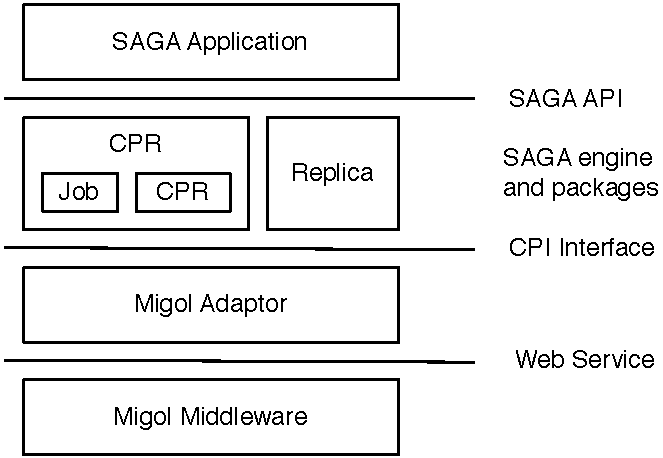
\includegraphics[width=0.6\textwidth]{saga-migol-layered}
%   \caption{SAGA Adaptor for Migol infrastructure}
%   \label{fig:saga-migol-layered}
% \end{figure}  


% \section{Experiences with a Large-Scale Task-Farming Application in the LONI Grid}
% \label{sec:exp}       
% 
%         
% %do we use checkpoints or do we automatically restart the task
% Figure~\ref{fig:saga-taskfarming} gives an overview about the task farming scenario. All tasks are
% distributed using a script and Migol's Job Broker Service.
% %  Each worker will compute a certain 
% % variation of the graph network. Depending on the graph size, the runtime of a single task  can 
% % be as high as \textbf{TODO}  days. 
% To enable the monitoring of a tasks, each task must initialize a \texttt{saga::session} object 
% before starting the computation.  Then, the Migol adaptor starts and registers the monitoring endpoint. 
% %TODO what is the task size/runtime of a single task
% The MRS can now monitor the application.  For error detection we use a timeout of 5 minutes.
% \begin{figure}[t]
%     \centering
%         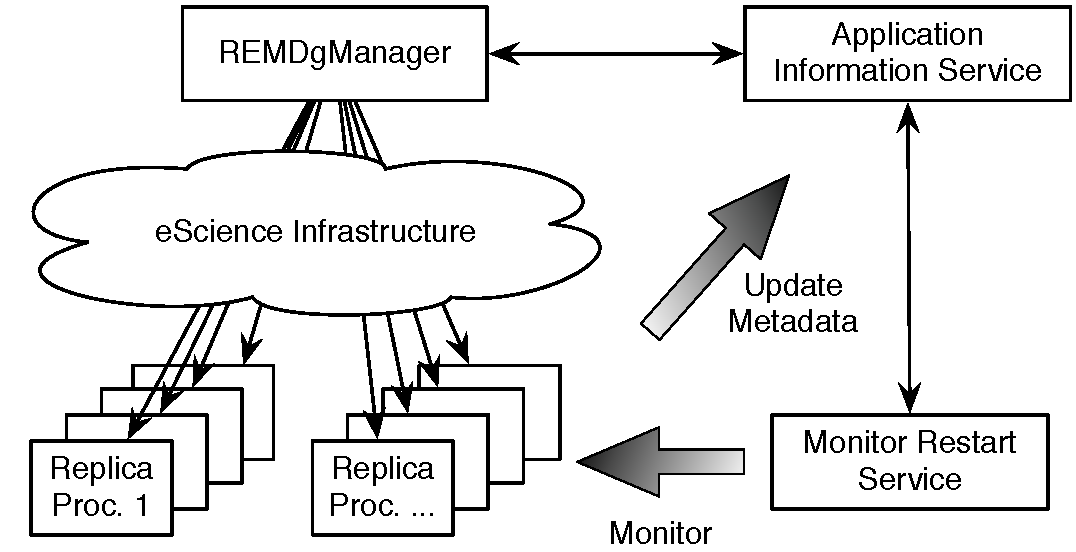
\includegraphics[width=\textwidth]{saga-taskfarming}
%     \caption{Fault Tolerant Task Farming Scenario}
%     \label{fig:saga-taskfarming}
% \end{figure}
% 
% 
% 
% 
%   
% 
% During the runtime, we simulate the failure of a number of worker
% processes.  The Migol MRS successfully detects the respective faults
% and recovers the worker nodes correctly. Even with a high failure
% rate, we were able to obtain the results of our computation.
